\chapter{Conservation of Mass and Energy}

One of the most fundamental laws in science is the conservation of mass and 
energy. This law states that mass (matter) and energy cannot be created or 
destroyed. This means the total matter and energy in the universe always stays 
the same. 

\section{Conservation of Mass}
Since matter cannot be created or destroyed, a chemical reaction does not change 
the mass of the reactants as they form products. Consider the reaction between 
vinegar and baking soda, which produces carbon dioxide, water, and sodium acetate:

\begin{center}
    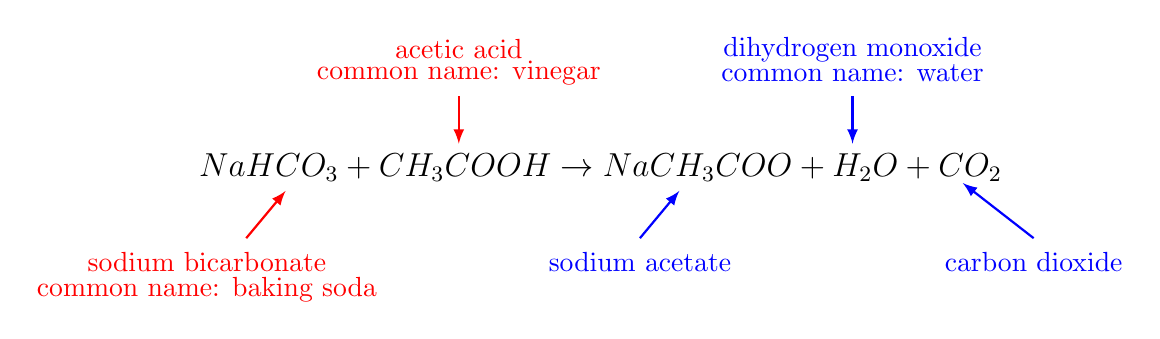
\begin{tikzpicture}
        \node[font = \large] at (0,0) {$NaHCO_3 + CH_3COOH \to NaCH_3COO + H_2O + CO_2$};
        \node[red] at (-5, -1.2) {sodium bicarbonate};
        \node[red] at (-5, -1.55) {common name: baking soda};
        \draw[thick, red, -latex] (-4.5, -0.9) -- (-4, -0.3);
        \node[red] at (-1.8, 1.2) {common name: vinegar};
        \node[red] at (-1.8, 1.5) {acetic acid};
        \draw[thick, red, -latex] (-1.8, 0.9) -- (-1.8, 0.3);
        \node[blue] at (0.5, -1.2) {sodium acetate};
        \draw[thick, blue, -latex] (0.5, -0.9) -- (1, -0.3);
        \node[blue] at (3.2, 1.5) {dihydrogen monoxide};
        \node[blue] at (3.2, 1.2) {common name: water};
        \draw[thick, blue, -latex] (3.2, 0.9) -- (3.2, 0.3);
        \node[blue] at (5.5, -1.2) {carbon dioxide};
        \draw[thick, blue, -latex] (5.5, -0.9) -- (4.6, -0.2);
    \end{tikzpicture}
\end{center}

The reactants are labeled with red, and the products with blue. This equation is
\textit{balanced}: that is, it shows the same number of each element on each side
of the arrow. This shows that the atoms are not created or destroyed during a 
chemical reaction; they are only rearranged. Take a minute to count up each 
element on each side. You should find there are 5 hydrogens, 1 sodium, 3 carbons,
and 5 oxygens on each side. 

Now, let's look at an \textit{unbalanced} chemical reaction. As you know, hydrogen
and oxygen combine to form water. Additionally: hydrogen and oxygen both exist as
\textit{diatomic gases}. When we say "oxygen gas" or "hydrogen gas", we mean the 
diatomic molecules, $O_2$ and $H_2$, respectively. Here is an unbalanced chemical 
reaction between hydrogen gas and oxygen gas to form water:

\begin{center}
    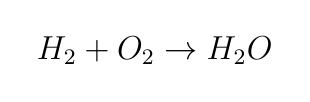
\begin{tikzpicture}
        \node[font = \large] at (0,0) {$H_2 + O_2 \to H_2O$};
    \end{tikzpicture}
\end{center}

How do we know this equation is unbalanced? Count up the elements: there are two 
oxygen atoms on the reactant side, but only one on the product side. This violates 
the conservation of matter: that oxygen atom cannot just disappear!

\subsection{Balancing Chemical Reactions}
We solve this by \textit{balancing} the chemical reaction: adjusting the number 
of products and reactants to comply with the Law of Conservation of Matter. You'll
learn strategies for balancing chemical reactions in Sequence 2, but for now we'll
briefly balance this chemical reaction so that it complies with the Law of 
Conservation of Matter. You may be tempted to simply add a lone oxygen atom to 
the products side:

\begin{center}
    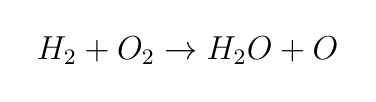
\begin{tikzpicture}
        \node[font = \large] at (0,0) {$H_2 + O_2 \to H_2O + O$};
    \end{tikzpicture}
\end{center}

The major reason this is incorrect is that oxygen does not exist as a lone atom -
as discussed above - so it doesn't make sense to have a lone oxygen as a product. 
So maybe we should add a molecule of oxygen gas to both sides?

\begin{center}
    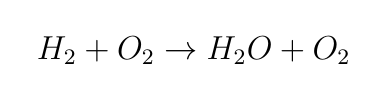
\begin{tikzpicture}
        \node[font = \large] at (0,0) {$H_2 + O_2 \to H_2O +O_2$};
    \end{tikzpicture}
\end{center}

Well now we have the same problem we started with: the oxygens are unbalanced. 
When balancing chemical reactions, we can only add \textit{whole molecules} that 
are already in the reaction. Let's take another look at our unbalanced reaction 
with some molecular models for visualization:

\begin{center}
    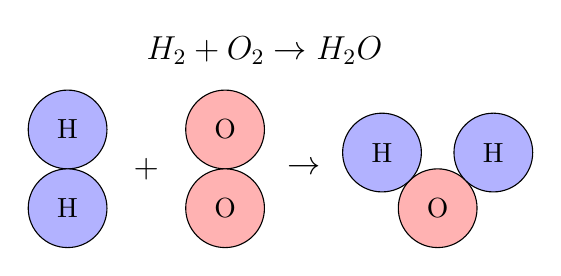
\begin{tikzpicture}
        \node[font = \large] at (0,0) {$H_2 + O_2 \to H_2O$};
        \draw[draw=black, fill=blue!30] (-2.5, -1) circle (0.5);
        \draw[draw=black, fill=blue!30] (-2.5, -2) circle (0.5);
        \node[] at (-2.5, -1) {H};
        \node[] at (-2.5, -2) {H};
        \node[font = \large] at (-1.5, -1.5) {+};
        \draw[draw=black, fill=red!30] (-0.5, -1) circle (0.5);
        \draw[draw=black, fill=red!30] (-0.5, -2) circle (0.5);
        \node[] at (-0.5, -1) {O};
        \node[] at (-0.5, -2) {O};
        \node[font = \large] at (0.5, -1.5) {$\to$}; 
        \draw[draw=black, fill=red!30] (2.2, -2) circle (0.5);
        \node[] at (2.2, -2) {O};
        \draw[draw=black, fill=blue!30] (1.493, -1.293) circle (0.5);
        \draw[draw=black, fill=blue!30] (2.907, -1.293) circle (0.5);
        \node[] at (1.493, -1.293) {H};
        \node[] at (2.907, -1.293) {H};
    \end{tikzpicture}
\end{center}

You can clearly see we need more oxygens on the product side. Since we can only 
add \textit{whole molecules}, our only option is to add another water. We do this
by adding a coefficient of 2 in front of $H_2O$ in our equation, which indicates 
2 water molecules (just like $2x$ means two x's):

\begin{center}
    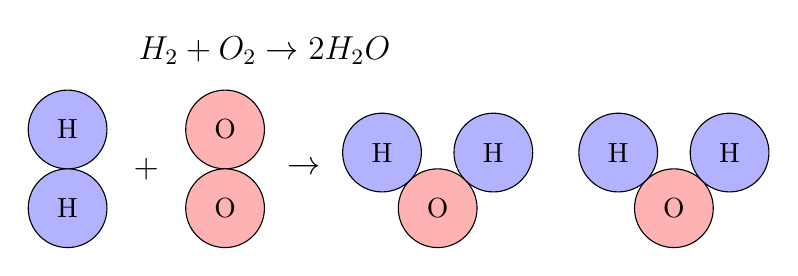
\begin{tikzpicture}
        \node[font = \large] at (0,0) {$H_2 + O_2 \to 2H_2O$};
        \draw[draw=black, fill=blue!30] (-2.5, -1) circle (0.5);
        \draw[draw=black, fill=blue!30] (-2.5, -2) circle (0.5);
        \node[] at (-2.5, -1) {H};
        \node[] at (-2.5, -2) {H};
        \node[font = \large] at (-1.5, -1.5) {+};
        \draw[draw=black, fill=red!30] (-0.5, -1) circle (0.5);
        \draw[draw=black, fill=red!30] (-0.5, -2) circle (0.5);
        \node[] at (-0.5, -1) {O};
        \node[] at (-0.5, -2) {O};
        \node[font = \large] at (0.5, -1.5) {$\to$}; 
        \draw[draw=black, fill=red!30] (2.2, -2) circle (0.5);
        \node[] at (2.2, -2) {O};
        \draw[draw=black, fill=blue!30] (1.493, -1.293) circle (0.5);
        \draw[draw=black, fill=blue!30] (2.907, -1.293) circle (0.5);
        \node[] at (1.493, -1.293) {H};
        \node[] at (2.907, -1.293) {H};

        \draw[draw=black, fill=red!30] (5.2, -2) circle (0.5);
        \node[] at (5.2, -2) {O};
        \draw[draw=black, fill=blue!30] (4.493, -1.293) circle (0.5);
        \draw[draw=black, fill=blue!30] (5.907, -1.293) circle (0.5);
        \node[] at (4.493, -1.293) {H};
        \node[] at (5.907, -1.293) {H};
    \end{tikzpicture}
\end{center}

We've fixed our oxygen problem: now there are two oxygen atoms on both sides. 
But now we have a hydrogen problem: there are 2 on the reactant side and 4 on 
the product side. We can address this by adding another hydrogen gas molecule 
to the reactant side:

\begin{center}
    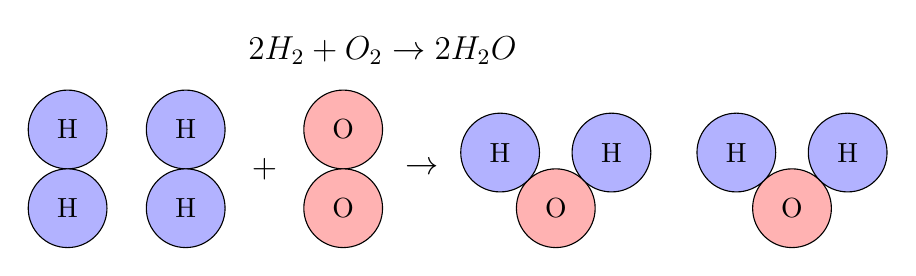
\begin{tikzpicture}
        \node[font = \large] at (0,0) {$2H_2 + O_2 \to 2H_2O$};
        \draw[draw=black, fill=blue!30] (-4, -1) circle (0.5);
        \draw[draw=black, fill=blue!30] (-4, -2) circle (0.5);
        \node[] at (-4, -1) {H};
        \node[] at (-4, -2) {H};
        
        \draw[draw=black, fill=blue!30] (-2.5, -1) circle (0.5);
        \draw[draw=black, fill=blue!30] (-2.5, -2) circle (0.5);
        \node[] at (-2.5, -1) {H};
        \node[] at (-2.5, -2) {H};
        \node[font = \large] at (-1.5, -1.5) {+};
        \draw[draw=black, fill=red!30] (-0.5, -1) circle (0.5);
        \draw[draw=black, fill=red!30] (-0.5, -2) circle (0.5);
        \node[] at (-0.5, -1) {O};
        \node[] at (-0.5, -2) {O};
        \node[font = \large] at (0.5, -1.5) {$\to$}; 
        \draw[draw=black, fill=red!30] (2.2, -2) circle (0.5);
        \node[] at (2.2, -2) {O};
        \draw[draw=black, fill=blue!30] (1.493, -1.293) circle (0.5);
        \draw[draw=black, fill=blue!30] (2.907, -1.293) circle (0.5);
        \node[] at (1.493, -1.293) {H};
        \node[] at (2.907, -1.293) {H};

        \draw[draw=black, fill=red!30] (5.2, -2) circle (0.5);
        \node[] at (5.2, -2) {O};
        \draw[draw=black, fill=blue!30] (4.493, -1.293) circle (0.5);
        \draw[draw=black, fill=blue!30] (5.907, -1.293) circle (0.5);
        \node[] at (4.493, -1.293) {H};
        \node[] at (5.907, -1.293) {H};
    \end{tikzpicture}
\end{center}

And now we have the same number of hydrogens and oxygens on each side! Notice we 
have all the same reactants and products that we started with, but now in ratios 
that reflect the conservation of matter. 

A final note: if atoms are in parentheses followed by a subscript, the subscript 
applies to every atom in the parentheses. For example, zinc nitrate, $Zn \left( 
NO_3 \right)_2$ is made of 1 zinc, 2 nitrogens, and 6 oxygens. 

\begin{Exercise}[title = {Balanced and Unbalanced Reactions}, label = balance]
Classify the following chemical reactions as balanced or unbalanced. If it is 
unbalanced, state what element(s) are not conserved. 
\begin{enumerate}
\item $NiCl_2 + 2NaOH \to Ni \left(OH \right)_2 + 2NaCl$
\item $HgO \to Hg + O_2$
\item $BaSO_4 + 2C \to 2BaS + CO$
\item $Cd \left( NO_3 \right)_2 + H_2S \to CdS + 2HNO_3$
\end{enumerate}
\end{Exercise}

\begin{Answer}[ref = balance]
\begin{enumerate}
\item balanced
\item unbalanced; oxygen
\item unbalanced; barium, sulfur, oxygen, and carbon
\item balanced
\end{enumerate}
\end{Answer}

\section{Conservation of Energy}
Just like matter, energy is also conserved: it cannot be created or destroyed, 
only change forms. You'll learn more about the types of energy in a subsequent 
chapter, Work and Energy. The transformation of energy from one type to another 
drives our modern world: your phone transforms electrical potential energy into 
light and sound energy, a nuclear power plant transforms nuclear energy to 
electrical energy, and your car transforms chemical potential energy (in the 
gasoline) into kinetic energy (motion).

\subsection{Friction, Heat, and Energy "Loss"}
Imagine rolling a ball across a flat surface: you have given the ball some 
kinetic energy in its motion. If the kinetic energy were conserved, the ball 
would keep rolling at the same speed forever, as long as it was on a flat 
surface. Experience tells us this isn't what happens: the ball will eventually 
come to a stop. Why doesn't this violate the Conservation of Energy?

Friction is the force that opposes motion: whenever you slide two objects past 
each other, friction transforms kinetic energy into heat. Rub the palms of your 
hands together. You should feel warmth, a product of the friction between your 
hands. As the ball in the example above rolls, it also experiences friction 
between itself and the ground. The friction slowly transforms the kinetic energy 
of the ball into heat, causing the ball to lose kinetic energy. When all of the 
ball's kinetic energy is transformed to heat, the ball comes to a rest. So, the 
kinetic energy of the ball wasn't destroyed and didn't disappear: it became heat. 

In fact, nearly all energy in the universe will eventually be transformed to heat,
resulting in the inevitable "heat death" of the universe. Here is a short video 
about heat, entropy, and the heat death of the universe: 
\url{https://www.youtube.com/watch?v=gOWt_Hq3yrE/}. 

\section{Types of Systems}
We classify systems based on the flow of matter and energy. A \textit{system} is 
a set of interconnected elements. Your body is a system, as is a television or a 
boiling pot of water. Scientists define systems by separating the parts of the 
system from the rest of the universe, usually called "the surroundings". You can 
represent this separation with a dashed line. Here is a diagram defining a pot of
boiling water as a system:

\begin{center}
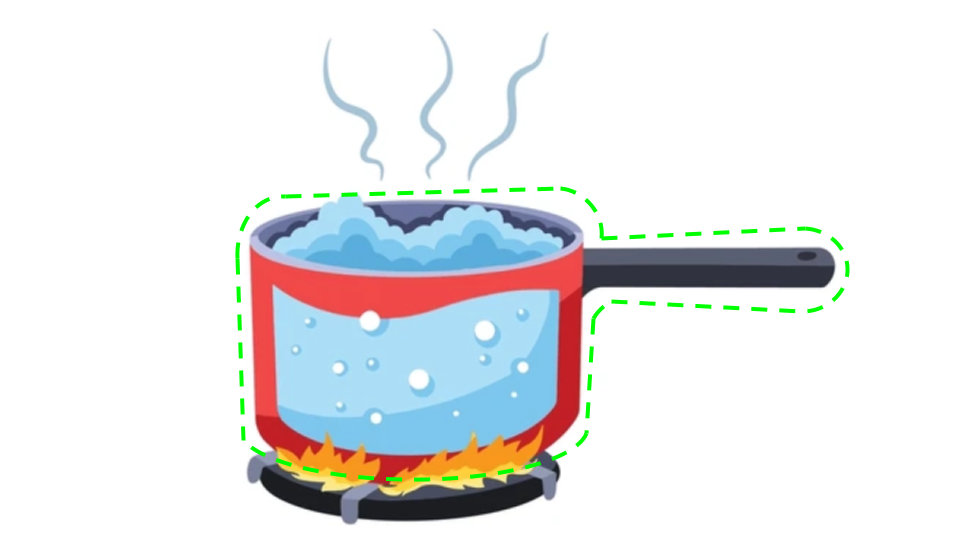
\includegraphics[width=4in]{pot_open_system.png}
\end{center}

Everything inside the dashed line is the system: the pot and the water boiling in
it. Everything outside the dashed line is the surroundings: the stove, the air 
around the pot, etc. Defining a system is \textit{arbitrary}: there isn't one hard 
and fast definition of a system. Think of your school: you could look at the 
system of a classroom, the system of a hallway and all the classes connected to 
it, or the entire school building. How you define a system depends on what you're 
studying. 

\subsection{Open Systems}
An \textit{open system} allows for matter and energy to cross the imaginary 
boundary between the system and its surroundings. The uncovered pot of boiling 
water is an example of an open system. Energy enters the system as heat from the
stove, and leaves the system as heat in the steam rising from the pot. Notice 
that steam rising: see how it crosses the imaginary boundary? The steam is matter 
\textit{leaving the system}. Since matter and energy can cross the boundary 
between the system and its surroundings, the uncovered boiling pot is an open 
system. \index{open system}

\begin{center}
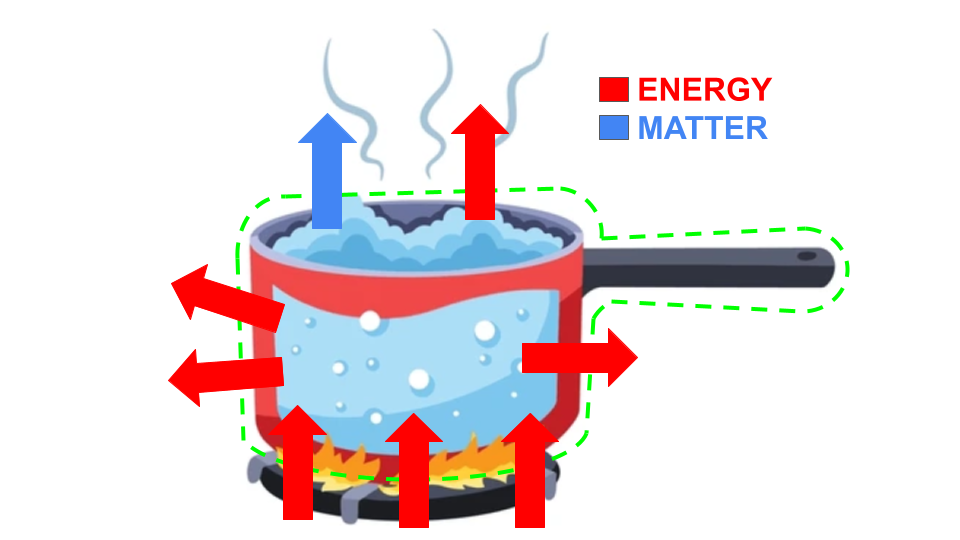
\includegraphics[width=4in]{pot_open_arrows.png}
\end{center}

The system also loses energy through the sides of the pot: if you touched the 
pot, it would feel hot, which means heat energy can also leave the system through
the sides of the pot. This is due to the collision between air particles (the 
surroundings) and the outside of the pot (the system). With every collision, a 
little heat is transferred from the pot to the air. This is why your hot drink 
gets cold if you leave it out, even if you don't add any ice. 

\subsection{Closed Systems}
A \textit{closed system} allows for the transfer of energy but not the transfer 
of matter. If we put a lid on this pot, it would become a closed system. 
\index{closed system}

\begin{center}
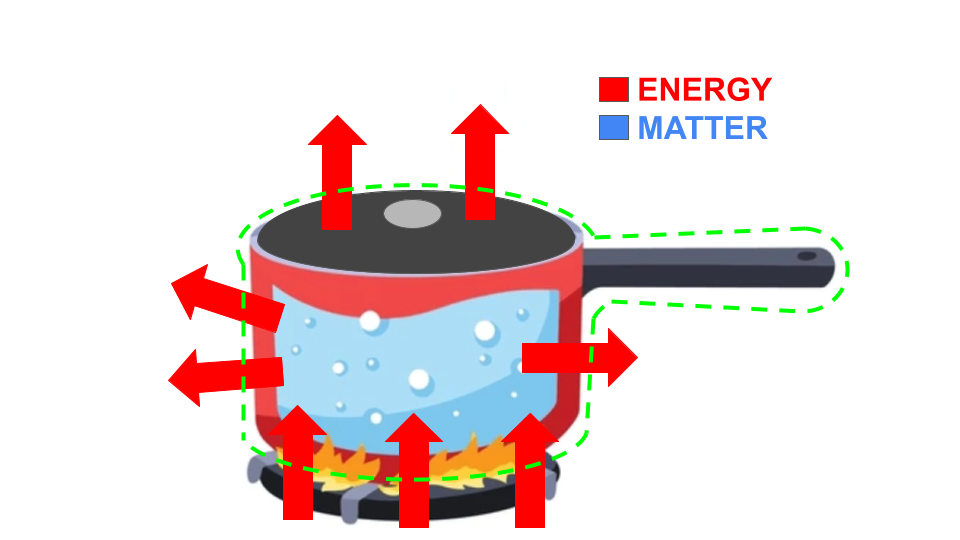
\includegraphics[width=4in]{pot_closed_system.png}
\end{center}

Notice that the difference between an open and closed system is the flow of 
\textit{matter}: open systems allow for the movement of matter, while closed 
systems do not. However, energy can still enter and leave closed systems. 
Sealed containers that aren't insulated are good examples of closed systems - 
a car with the windows up and doors closed. 

\subsection{Isolated Systems}
An \textit{isolated system} does not allow for the flow of matter \textit{or} 
energy in or out of the system. There is no such thing as a truly isolated system
- in reality a small amount of energy can be transferred even through the best 
thermal insulators. However, for well-insulated systems, it can be a good 
approximation to model that system as isolated. A simple example would be a 
sealed, well-insulated coffee thermos. The transfer of heat energy between the 
coffee in the thermos and the thermos' surroundings is so slow that we can ignore
that small amount of transfer and approximate the thermos as an isolated system. 

\subsection{Classifying Systems}
To quickly categorize a system as open, closed, or isolated, ask yourself two questions:
\begin{enumerate}
\item Can matter enter or leave the system?
\item Can energy enter or leave the system?
\end{enumerate}

If your answer to the first question is yes, you know automatically the system 
is open. If no, move to the second question. If energy can enter or leave, the 
system is closed. If not, the system is isolated. Sometimes, textbooks and exams 
will describe a system as "well-insulated". This is directing you to assume any 
transfer of energy between the system and surroundings is negligible, and that 
you should treat the system as an isolated system. 

\begin{Exercise}[title = {Open, Closed, and Isolated Systems}, label = systems]
Classify each system as open, closed, or isolated. Justify your answer. 
\begin{enumerate}
\item The human body
\item Earth
\item Your cell phone
\item A well-insulated cooler with the lid sealed
\item A well-insulated cooler with the lid open
\item A bottle of soda before it is opened to be drunk
\end{enumerate}
\end{Exercise}

\begin{Answer}[ref = systems]
\begin{enumerate}
\item The human body is an open system because matter can enter (food, water, 
oxygen) and leave (waste, carbon dioxide, sweat) your body.
\item The Earth is an open system because matter can enter (asteroids falling, 
spaceships returning) and leave (space vehicles and astronauts). On the other 
hand, the Earth can be well-approximated as a closed system. Before the 20th 
Century, humans had no way to deliberately expel matter from the Earth, and the 
mass of asteroids that are pulled in by the Earth's gravity is negligible 
compared to the Earth. Therefore, in the right circumstances, it would be 
appropriate to model the Earth as a closed system. (It is closed because 
energy in the form of sunlight is constantly entering the system.)
\item A cell phone is a closed system - you don't put any matter in or take it 
out of your phone, but it constantly uses battery and then is recharged, showing
that energy enters and leaves your phone. 
\item Since the cooler is described as well-insulated and the lid is closed, it 
can be approximated as an isolated system. Scientific equipment, like bomb 
calorimeters, rely on this approximation. 
\item With the lid open, matter can enter and leave and therefore the cooler is 
an open system (yes, even though it is well-insulated). 
\item A sealed bottle of soda is a closed system - the soda and carbon dioxide 
can't escape, but energy in the form of heat can be transferred in and out of 
the system (the contents of the bottle will lose heat if you put it in the 
fridge and gain heat if you leave it in the sun).
\end{enumerate}
\end{Answer}